% ME3050 -  Dynamics Modeling and Controls - Tennessee Technological University
% Tristan Hill - Spring 2020 - Summer 2020 - Spring 2022
% Dynamics Modeling and Controls
% Lecture Module - Newtons Approach  - Topic 1 - Newton's Three Laws  
% Document settings

%\documentclass{beamer}                  % for presentation ?
\documentclass[handout]{beamer}  % for handout ?

\usepackage{/home/thill/Documents/lectures/dmc_lectures/dmc_lectures}

\newcommand{\MNUM}{3\hspace{2mm}} % Module number
\newcommand{\TNUM}{2\hspace{2mm}} % Topic number 
\newcommand{\moduletitle}{Newton's Approach}
\newcommand{\topictitle}{Equations of Motion} 

\newcommand{\sectiontitleI}{Modeling Rigid Body Mechanical Systems}
\newcommand{\sectiontitleII}{Derive Equations of Motion}
\newcommand{\sectiontitleIII}{Newton's Second Law Approach}
\newcommand{\sectiontitleIV}{Convervation of Energy Method}

\author{ME3050 - Dynamic Modeling and Controls}
\title{Lecture Module - \moduletitle}
\date{Mechanical Engineering\vspc Tennessee Technological University}

\begin{document}
	
	\lstset{language=MATLAB,basicstyle=\ttfamily\small,showstringspaces=false}
	
	\frame{\titlepage \center\begin{framed}\Large \textbf{Topic \TNUM - \topictitle}\end{framed} \vspace{5mm}}
	
	% Section 0 - Outline
	\frame{
		
		\large \textbf{Topic \TNUM - \topictitle} \vspace{3mm}\\
		
		\begin{itemize}
			
			\item \sectiontitleI    \vspc % Section I
			\item \sectiontitleII 	\vspc % Section II
			\item \sectiontitleIII 	\vspc %Section III
			\item \sectiontitleIV 	\vspc %Section IV
			%\item \sectiontitleV 	\vspc %Section V
			
		\end{itemize}
		
	}

% Section I:
\section{\sectiontitleI}

\frame{
\frametitle{\sectiontitleI}

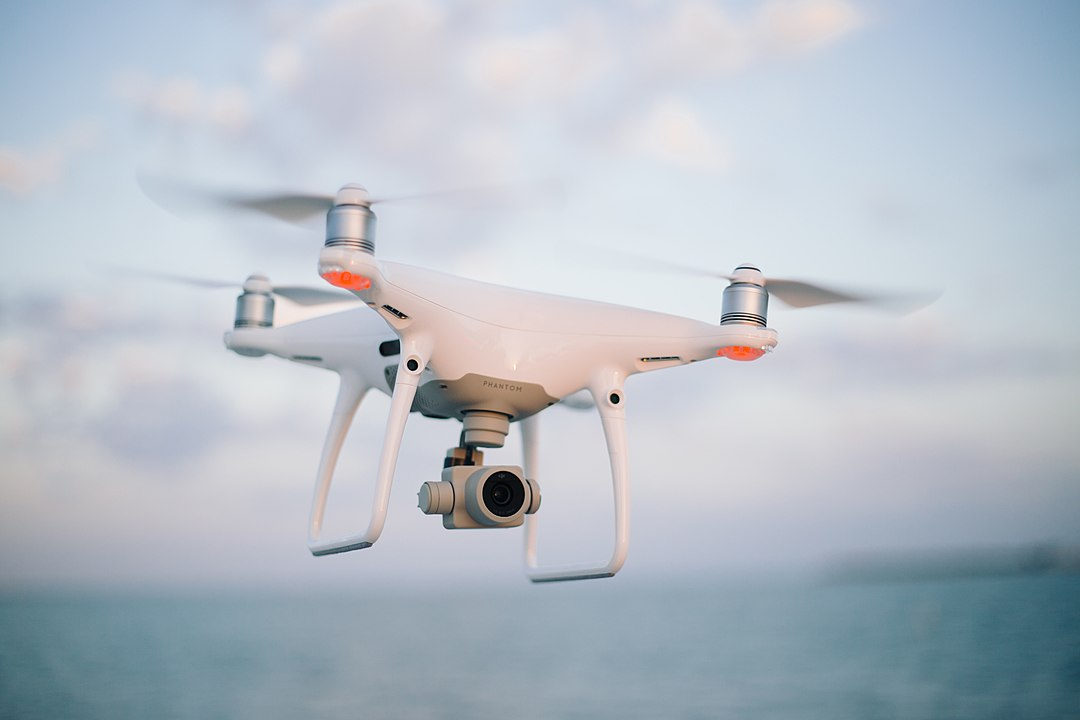
\includegraphics[scale=.1]{quadcopter.jpg} 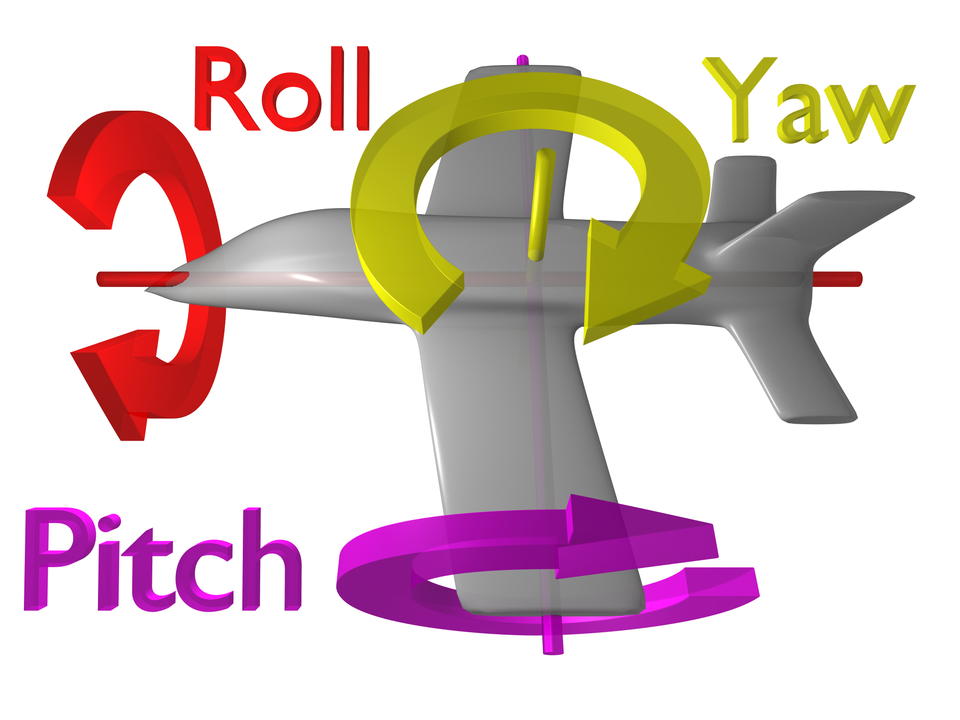
\includegraphics[scale=.10]{flight_dynamics.png}

{\it When modeling the motion of objects, the bending or twisting of the object is often negligible, and we can model the object as a rigid body. We begin this chapter by reviewing Newton's laws of motion and applying them to rigid bodies where the object;s motion is relatively uncomplicated, simple translations and simple rotations about a fixed axis.} {\tiny \underline{System Dynamics, Third Edition}, Palm - Pg. 117} 


}

% Section II:
\section{\sectiontitleII}

\frame{
\frametitle{\sectiontitleII}

To analyze the dynamics (motion and forces) of a system we start by deriving the {\B equations of motion} (EOM). This is typically done in one of two ways. \vspc

\begin{itemize}
	\item  \vspace{3mm}
	\item  \vspace{3mm}
\end{itemize}
\vspace{3mm}
The \hspcu \hspcu \hspcu are \hspcu\hspcu\hspcu describing the dynamic relationships between the bodies in the system.
}

% Section III:
\section{\sectiontitleIII}

\frame{
\frametitle{\sectiontitleIII}

To derive the equations of motion with Newton's Second Law:
\begin{enumerate}
\item Draw a {\PR free body diagram} (FBD) for each body in the system. Identify all forces acting on the bodies in the system. \vspc
\item Apply Newton's Second Law for each {\PN DOF}. 
\end{enumerate}

\begin{tabular}{ccc}
Translation:&$\Sigma {\bf F}=m{\bf a}$&$ \Sigma F_x=ma_x$\\
&&$\Sigma F_y=ma_y$\\
&&$\Sigma F_z=ma_z$ \\
&&\\
Rotation: &$\Sigma {\bf M}=I_o{\bf \alpha}$&$\Sigma M_o=I_o\alpha_z$\\
\end{tabular}
}

% Section IV:
\section{\sectiontitleIV}

\frame{
\frametitle{\sectiontitleIV}

Alternatively with Conservation of Energy:

\begin{enumerate}
\item Draw a {\PR free body diagram} (FBD) for each body in the system. Identify all {\R kinetic} and {\B potential} energies present in the system.

\item Write the {\BR total energy} equation as the sum of all energies for a particular body.



\item If no \hspcu forces are considered, Conservation of Energy states the change in the \hspcu must equal zero. \hspcu\hspcu\hspcu\hspcu. This relation is used to the derive the EOM(s).\vspc
\end{enumerate}

}
	
\frame{
\frametitle{\sectiontitleIV}

\textbf{Note:}\vspc

Either method can be used and for some problem types one or the other is preferred. We will look at several examples of both but the course will primarily focus on the Newton's Second Law approach. \vspc

The Conservation of Energy method, which is based upon Newton's law, is commonly used in advanced dynamics courses. \\


}	
	
	
\end{document}





